\minpurp{Muster Allgemein}
Lösungsschablone zur Lösung eines Problems, in der Praxis bewährt

\minpurp{Architekturmuster}
Vorraussetzung: Modularität

\minmeth{Model-View-Controller}
Darstellung von variablen Daten in verschiedenen Sichten

Leichte Änderbarkeit der Views => Unabhängig vom Kern implementiert;

Direke Anpassung der Sichten bei Änderungen

\submeth{Lösung}
Modularisierung:

Model: Kernfunktionalität und Datenmodell; registriert und informiert View u. Controller

View: Darstellung der vom Model abgefragten Daten

Controller: Auswertung Benutzereingaben => Aufruf von Model bzw. Viewfunktionen

Bei Implementierung: 

Observer Pattern: Observable->Model, Observer->View,Controller

Command Pattern: Aufrufer->View, Befehl->Controller (Interface) Konkreter Befehl->ControllerImpl.

\minpurp{Design Pattern}
Vorraussetzung: Objektorientierung

\quarterpage{
\minmeth{Strategy} Austauschbare Algorithmen

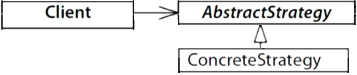
\includegraphics[width=0.9\textwidth]{strategy}
}
\quarterpage{
\minmeth{Iterator} Sequentieller Zugriff auf Elemente eines Aggregats ohne interna preiszugeben. 

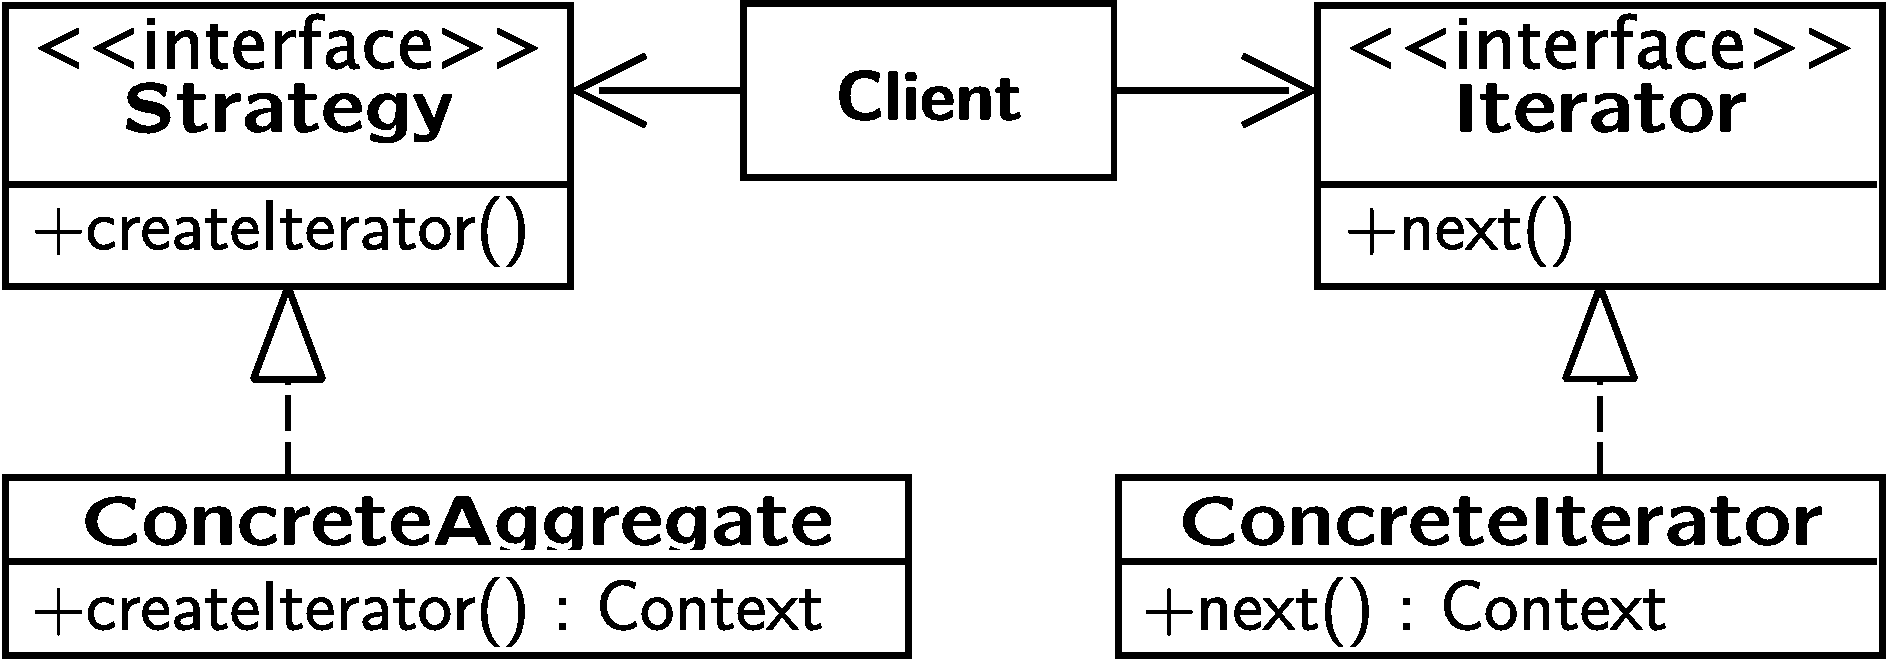
\includegraphics[width=0.9\textwidth]{iterator}
}

\halfpage{
\minmeth{Observer} Informieren von Objekten über Zustandsänderungen eines Objektes
Varianten:

Pull: keine information im notify

Push: Zustandsänderung wird mitgeschickt

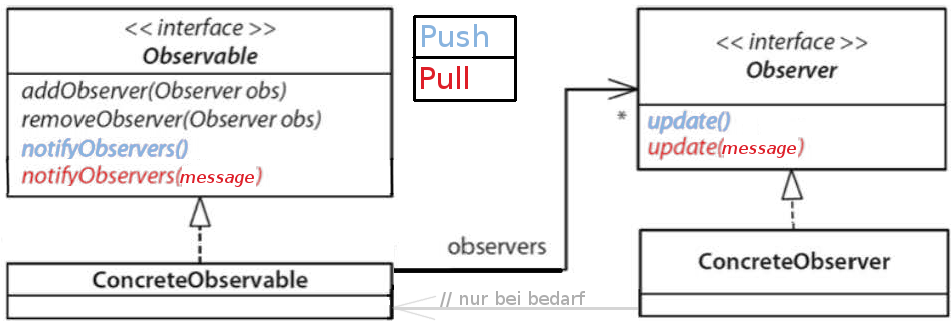
\includegraphics[width=0.6\textwidth]{observer}
}

\halfpage{
\divpage{
\minmeth{Composite} Hierarchiestruktur, 

Verwendung der Teile unabhängig von der Position (Knoten vs Blatt)

Lösung: Schnittstelle mit Operationen für Hierarchieverwaltung und Elementfunktionen

=> Keine Unterschiede für Client
}\divpage{ ~~~~

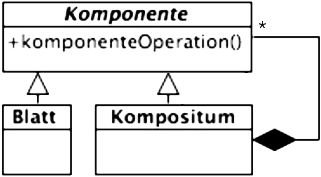
\includegraphics[width=0.9\textwidth]{Composite}
}
}

\halfpage{
\minmeth{Factory Method}

Problem: Objekt erzeugen. Nur Schnittstelle nicht konkrete Klasse bekannt. 

Factory Method: Hook für Subklasse, um Verhalten in der Basisklasse zu konfigurieren. Product und Creator bilden häufig „parallele“ Klassenhierarchien.
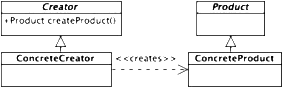
\includegraphics[width=0.6\textwidth]{factory}
}

\halfpage{
\minmeth{Abstract Factory}

entkopplung Objekterzeugung/-verwendung. Factory Method legt Klasse der Objekte fest. 
(Delegieren Objekterzeugung)

Factory Instanzen implementieren Factory Methoden für Objekte einer Klassenfamilie

Schnittstelle AbstractFactory sieht eine Factory Methode je
Produkt vor. Definiere pro Produktfamilie eine ConcreteFactory Klasse

=> System arbeitet unabhängig von Objekterzeugung. Austausch
von Produktfamilien ist einfach. Schwierig, neue Produkte einzuführen, da alle
Factoryklassen um eine Methode ergänzt werden müssen.

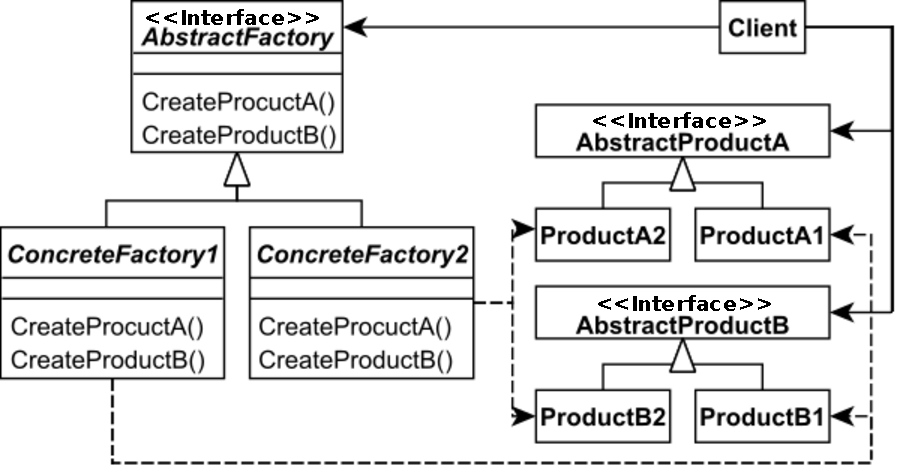
\includegraphics[width=0.7\textwidth]{abstractfactory-eps-converted-to}
}

\halfpage{
\minmeth{Adapter}
Client erwartet andere Schnittstelle als Service bietet (z.B. Legacy)

=> Adapter Zwischenobjekt

Implementierungen: 

\halfpage{
class Adapter

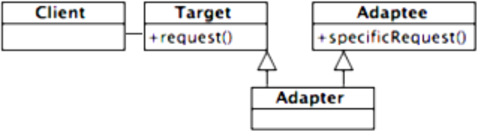
\includegraphics[width=0.9\textwidth]{adapterclass}
}
\halfpage{
object Adapter

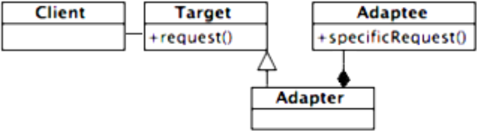
\includegraphics[width=0.9\textwidth]{adapterdelegate}
}

\submeth{Vergleich}Schnittstelle, welche verschieden vom Service Objekt ist.

Varianten: Two-Way-Adapter: Adapter bietet beide Schnittstellen an

Adapt Interface: Klasse implementiert nicht alle methoden der Schnittstelle => adapter liefert default implementierung.

}

\halfpage{
\begin{minipage}{0.6\textwidth}
\minmeth{Proxy}
Bei teurem Zugriff auf Service Objekt (z.B nur bei Bedarf erzeugen u. initialisieren)

Entkopplung des Aufrufs durch Zwischenobjekt

\submeth{Vergleich}Proxy Implement gleiche Schnittstelle wie Service Objekt.
\end{minipage}
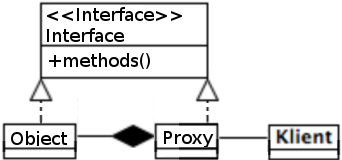
\includegraphics[width=0.4\textwidth]{proxy}
}

\halfpage{
\divpage{
\minmeth{Dekorator}
Funktionalität von Instanzen erweitern, ohne Klasse zu verändern

=> Objekt in Dekorator kapseln 

\submeth{Vergleich} Schnittstelle, welche die des Service Objekts erweitert.
}
\divpage{ ~

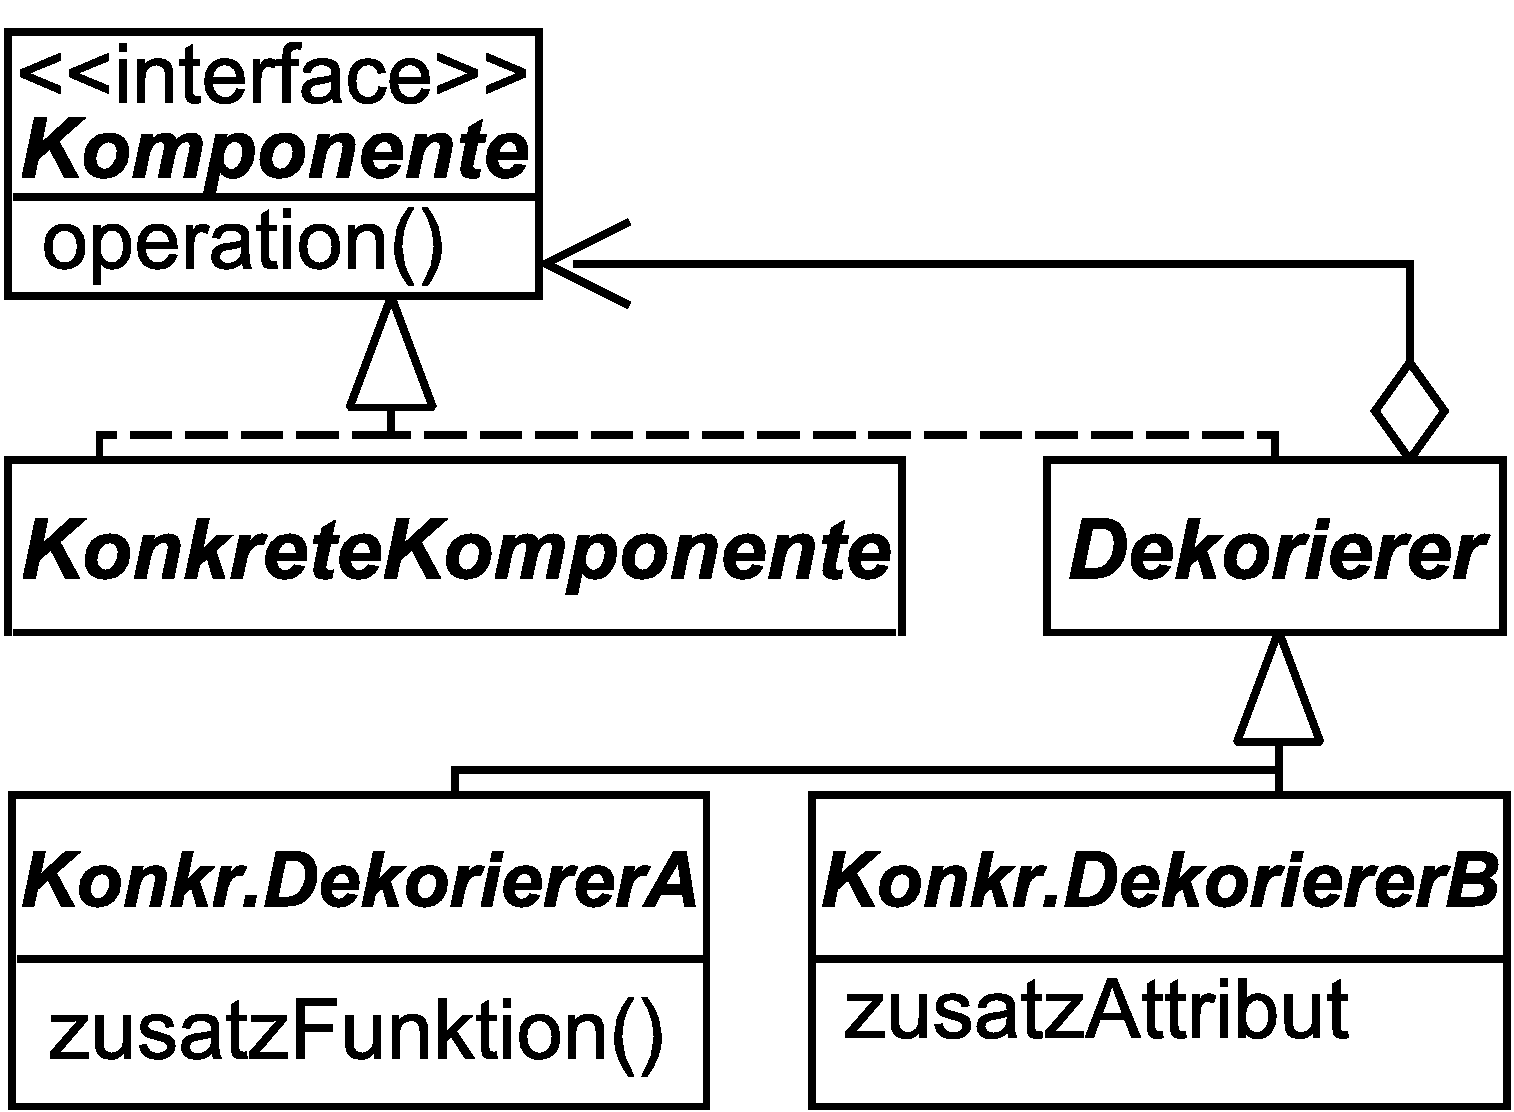
\includegraphics[width=0.8\textwidth]{Dekorator}
}
}

\halfpage{
\minmeth{Facade}

Client interagiert mit vielen Schnittstellen eines Subsystems => erhöhte Kompexität und Abhängigkeiten => Zusammenfassen in einem Objekt
}

\halfpage{
\minmeth{Command}
kapselung von Operation mit Kontext z.B. für Queueing, entkoppeln auswahl/ausführen (z.B. in anderem Thread), gruppieren von Operationen 

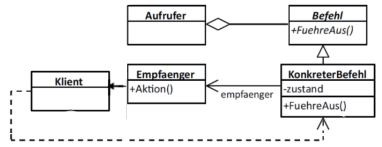
\includegraphics[width=0.6\textwidth]{Command}

}
\halfpage{
\divpage{\minmeth{Singleton}
Nur eine Instanz der Klasse, globaler Zugriffsmechanismus 

=> statische Fabrikmethode getInstance; private Konstruktoren; 
}\divpage{~ 

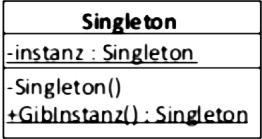
\includegraphics[width=0.5\textwidth]{Singleton}
}
}

\minpurp{Programmieridiome}
Vorraussetzung: Konkrete Sprache

\minmeth{Mixin} Erweitert bestehende Klasse ohne Vererbung zu verändern\\
\textcolor{mehrblau}{ohne Mehrfachvererbung}, \textcolor{mehrred}{mit Mehrfachvererbung}\\
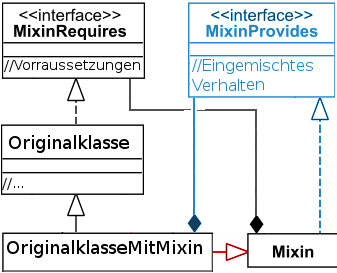
\includegraphics[width=0.24\textwidth]{mixinjava}


